\documentclass{beamer}
\beamertemplatenavigationsymbolsempty
\usecolortheme{beaver}
\setbeamertemplate{blocks}[rounded=true, shadow=true]
\setbeamertemplate{footline}[page number]
%
\usepackage[utf8]{inputenc}
\usepackage[english,russian]{babel}
\usepackage{amssymb,amsfonts,amsmath,mathtext}
\usepackage{subfig}
\usepackage[all]{xy} % xy package for diagrams
\usepackage{array}
\usepackage{multicol}% many columns in slide
\usepackage{hyperref}% urls
\usepackage{hhline}%tables
% Your figures are here:
\graphicspath{ {fig/} {../figures/} }

%----------------------------------------------------------------------------------------------------------
\title[\hbox to 56mm{Оптимальные методы оптимизации первого порядка с относительным шумом}]{Оптимальные методы оптимизации первого порядка с относительным шумом}
\author[Д.\,Н. Рубцов]{Денис Николаевич Рубцов}
\institute{Московский физико-технический институт}
\date{\footnotesize
\par\smallskip\emph{Курс:} Автоматизация научных исследований\par (практика, В.\,В.~Стрижов)/Группа 105
\par\smallskip\emph{Эксперт:} к.ф.-м.н. Э.\,А.~Горбунов
\par\smallskip\emph{Консультант:} Н.\,М.~Корнилов
\par\bigskip\small 2024}
%----------------------------------------------------------------------------------------------------------
\begin{document}
%----------------------------------------------------------------------------------------------------------
\begin{frame}
\thispagestyle{empty}
\maketitle
\end{frame}
%-----------------------------------------------------------------------------------------------------
% \begin{frame}{Цель исследования}
%\begin{block}{Решается задача}
%\end{block}
% \end{frame}
%-----------------------------------------------------------------------------------------------------
\begin{frame}{Доклад с одним слайдом}
\begin{equation}\label{formula_for_a}
    a = C \cdot \max{\{1, N^p \hat{\varepsilon}^2\}},\ C = 2304
\end{equation}
\begin{equation}\label{eq:conv_rate_alg1_proper_a}
\tau^N = f(y^N) - f(x^*) \leq 8C \cdot \max \left\{ \frac{LR_0^2}{N^p}, \hat{\varepsilon}^2 L R_0^2 \right\}.
\end{equation}

\begin{columns}[c]
\column{0.5\textwidth}
\begin{figure}
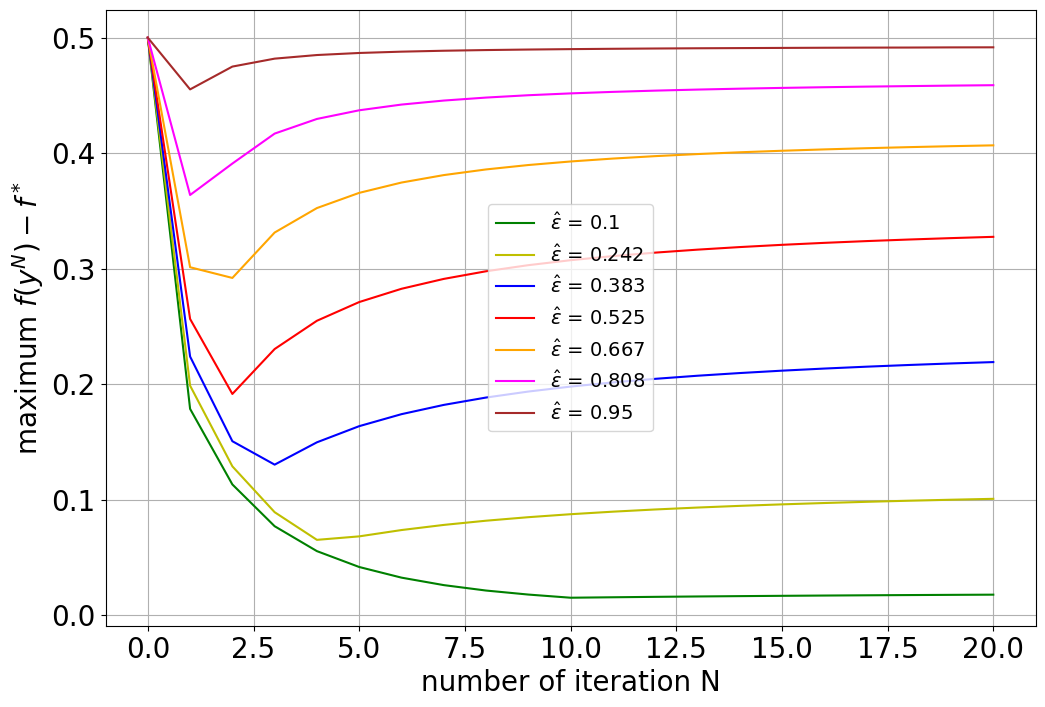
\includegraphics[width=1.0\textwidth]{convergence_rate.png}
    \caption{Графики зависимостей $\tau^N$  $N$ алгоритма \texttt{ISTM} для различных шумов $\hat{\varepsilon}$}
\end{figure}
\column{0.5\textwidth}
\begin{figure}
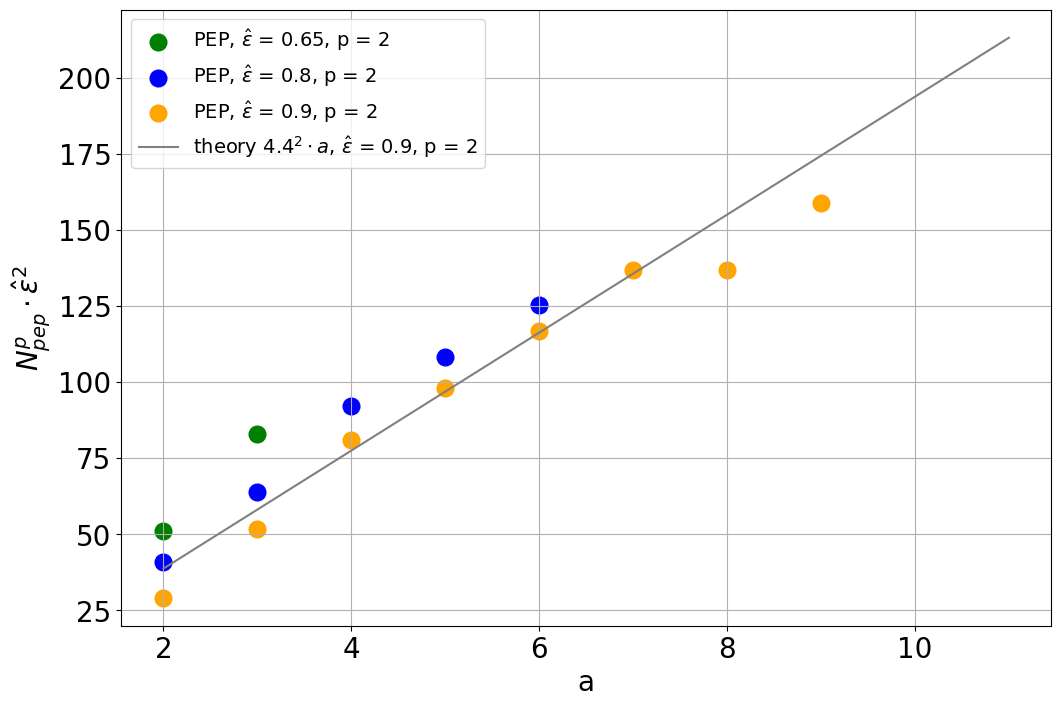
\includegraphics[width=1.0\textwidth]{find_c.png}
    \caption{Графики зависимости номера итерации расходимости метода $N_{pep}$ от $a$ для разных значений шума $\hat{\varepsilon}$. }
    \end{figure}
\end{columns}

\end{frame}


%----------------------------------------------------------------------------------------------------------
% \begin{frame}{Постановка задачи}
%
% \end{frame}
%----------------------------------------------------------------------------------------------------------
% \begin{frame}{Решение}
% \begin{columns}[c]
% \column{0.6\textwidth}
%     Столбец 1
% \column{0.4\textwidth}
%     Столбец 2
% \end{columns}
% \end{frame}
%----------------------------------------------------------------------------------------------------------
% \begin{frame}{Вычислительный эксперимент}
%
%  Что зритель видит на графике.
%
% \includegraphics[width=0.8\textwidth]{ErrorFunction}
%
% О чем говорит этот график.
%
% \end{frame}
%----------------------------------------------------------------------------------------------------------
% \begin{frame}{Заключение}
%     \begin{block}{Перечислите ваши результаты}
%     \begin{itemize}
%         \item предложен метод,
%         \item доказана теорема.
%     \end{itemize}
%     \end{block}
% \end{frame}
%----------------------------------------------------------------------------------------------------------

\end{document} 
